\documentclass{article}
\RequirePackage{amsmath}
\RequirePackage{amssymb}
\RequirePackage{wasysym} % for symbols
\RequirePackage{graphicx}
\RequirePackage{hyperref}
\RequirePackage{wrapfig}
\RequirePackage{xfrac}
\RequirePackage[utf8]{inputenc}

\title{Global addresses}
\author{}
% \author{Riccardo Gherardi \\ riccardo.gherardi@gmail.com}

\begin{document}

\maketitle
\begin{abstract}
What follows was an attempt to derive a mapping from a latitude / longitude pair to a single location identifier. The solution investigated below used regular subdivision and can not guarantee all the indexed Voronoi cells to have equal area. A better solution would be to create an equally spaced spiral on a sphere and divide it in equal segments (see \cite{lenofspherespiral, spherespiralmodel, pointsonsphere}). This is likely the solution W3W uses, coupled with a 45 bits identifier (3 words from a $2^{15}$ database, see \cite{effdice,diceware,PGPwordlist} for wordlists). Best option available today is plus codes \cite{plucodes, evaluation, opencodes}: they rely on an existing point of reference and allow to specify a variable length code for fine positioning within the area of interest. Realistically, an address should be capable of disambiguate an area at most the extent of Sahara desert, or metropolitan Tokyo.
%Coverage of water vs emerged lands
\end{abstract}

\section{How many identifiers are needed?} % ---- ---- ---- ---- ---- ---- ----

\begin{wrapfigure}{r}{0.3\textwidth}
\begin{center}
\vspace{-3.5em}
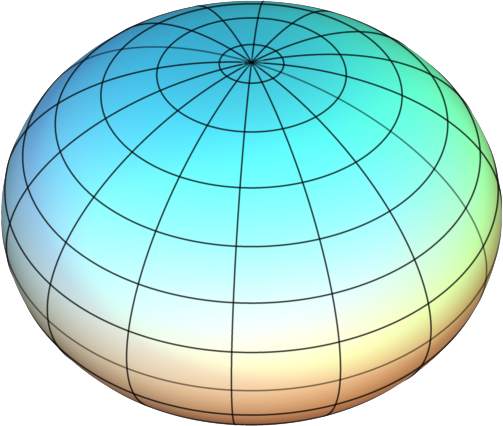
\includegraphics[width=0.25\textwidth]{oblateSpheroid.png}
\vspace{-2em}
\end{center}
\end{wrapfigure}
%
Coordinates on planet Earth can be specified with a latitude/longitude pair of numbers, which express location as a polar mapping on a reference sphere. Earth is more similar to an oblate spheroid, however GPS coordinates provide a convenient layer of abstraction over its actual geometry.

The surface area of Earth $A_E$ is roughly 510.1 million $\text{Km}^2$.
With each additional bit of information, we can halve the area we can index.
When using $B$ bits, the following relations hold:
%
\begin{align}
A_E &= 510.072 \cdot 10^{12} \text{ m}^2 &
A &= \frac{A_E}{2^B} &
B &= \log_2 \left( \frac{A_E}{A} \right)
\label{eq:nobits}
\end{align}
%
where $A$ is the area of each individual indexed patch.
Consumer GPS module have a worst case precision of 8-10 meters, however in normal usage 5 meters is the expected deviation from the true position. With temporal integration, is not uncommon for commercial units to deviate less than 3 meters from the true position in ideal conditions. Plugging into eq.~\ref{eq:nobits} the area of a circle of radius 3 meters, we obtain:
%
\begin{align*}
B &= \log_2 \left( \frac{A_E}{\pi R^2} \right) = \log_2 \left( \frac{510.072 \cdot 10^{12}}{\pi \; 3^2} \right) \gtrapprox 44.036 \text{ bits}
\end{align*}
%
which is a lower bound estimate of the bit budget required, since it is not possible to cover (tessellate) a surface exactly with circles.

\section{Regular subdivision}

One option to partition the surface of Earth into a number congruent shapes is to recursively subdivide a convex regular polyhedron inscribed in the reference sphere. This class of shapes is also known as platonic solids.
%
\begin{figure}[htb]
\centering
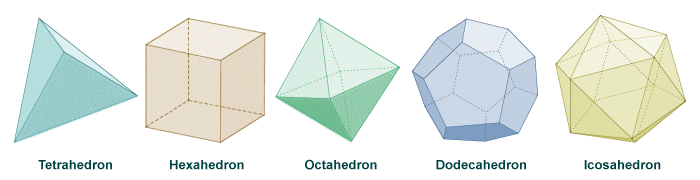
\includegraphics[width=0.9\textwidth]{platonic.png}
\end{figure}
%
All shapes but the dodecahedron have triangular or square faces, which can be conveniently subdivided into four equally sized and congruent pieces. We will ignore the dodecahedron for the rest of this document. A location can then be approximated providing an index to the closest face midpoint or vertex after subdivision.

It should be noted that regular subdivision does not guarantee equal areas; the discrepancy between the largest and smallest of them depend on the initial maximum distance between a point on the solid and the circumscribed sphere (e.g. largest on a tetrahedron, smallest for an icosahedron).

\subsection{Number of faces and vertexes after subdivision}

After $i$ rounds of subdivision, the following equations specify the total number of faces $F_i$, edges $E_i$ and vertexes $V_i$.
%
\begin{align}
F_i &= F_0 \cdot 4^i \label{eq:fcount} \\
E_i &= \frac{\mathcal{L}}{2} \cdot  F_i = \frac{\mathcal{L}}{2} \cdot F_0 \cdot 4^i = E_0 \cdot 4^i \label{eq:ecount} \\
V_i &= 2 + E_i - F_i = \notag \\
    &= 2 + \frac{\mathcal{L}}{2} \cdot F_i - F_i = 2 + \left( \frac{\mathcal{L}}{2} - 1 \right) \cdot F_i = \notag \\
    &= 2 + \frac{1}{2} \cdot (\mathcal{L} - 2) \cdot F_0 \cdot 4^i = 2 + \mathcal{V} \cdot 4^i \label{eq:vcount}
\end{align}
%
where $\mathcal{L}$ is the number of face edges and $\mathcal{V}$ is defined as $\sfrac{1}{2} (\mathcal{L} - 2) F_0$. Table~\ref{tab:polyfacts} summarizes the initial values for $i=0$.
%
\begin{table}[htb]
\centering
%\begin{center}
%\begin{wraptable}{r}{0.34\textwidth}
\begin{tabular}{ r c c c c c }
 & $V_0$ & $E_0$ & $F_0$ & $\mathcal{L}$ & $\mathcal{V}$ \\
\textbf{T}etrahedron & 4 & 6 & 4 & 3 & 2 \\
\textbf{C}ube, hexahedron & 8 & 12 & 6 & 4 & 6 \\
\textbf{O}ctahedron & 6 & 12 & 8 & 3 & 4\\
\textbf{I}cosahedron & 12 & 30 & 20 & 3 & 10
\end{tabular}
\caption{platonic solids statistics.}
\label{tab:polyfacts}
%\end{wraptable}
%\end{center}
\end{table}

\subsection{Tessellation types}

If using face midpoints to approximate locations, faces are subdivided into triangles or squares. When using vertexes, they are partitioned with the respective dual tessellations, hexagons and squares.

\begin{figure}[tbp]
    \centering
    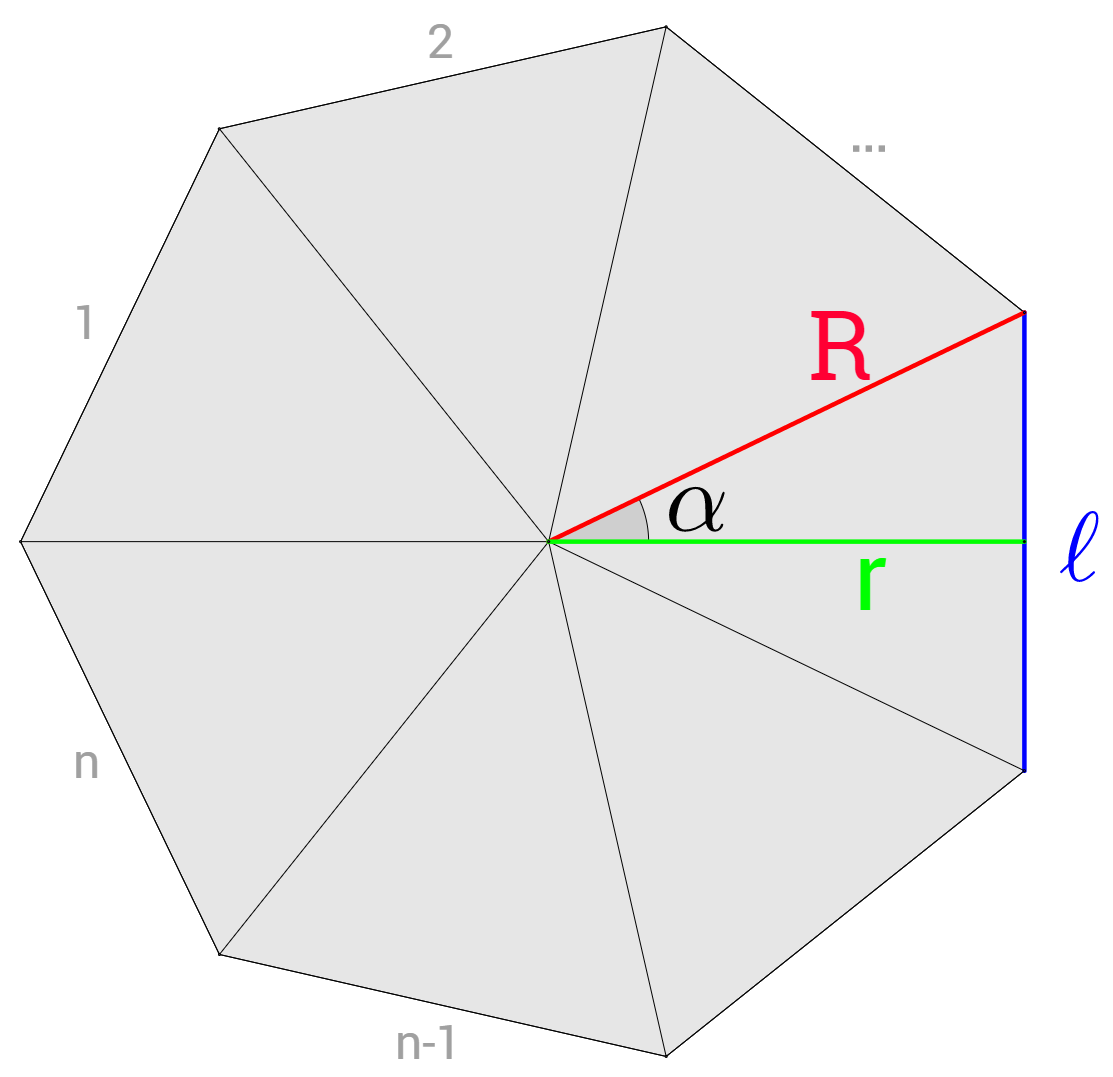
\includegraphics[width=0.32\textwidth]{polygon.png}
    \hspace{1em}
    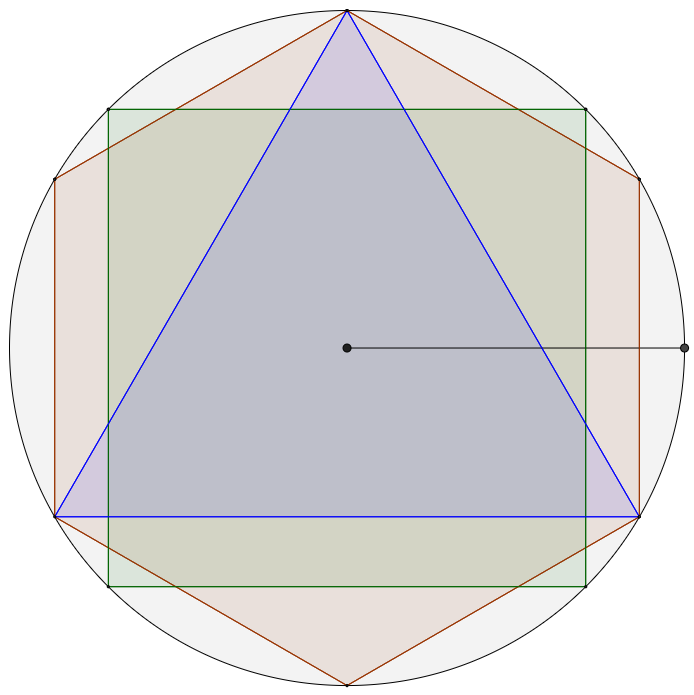
\includegraphics[width=0.305\textwidth]{areas.png}
    \hspace{1em}
    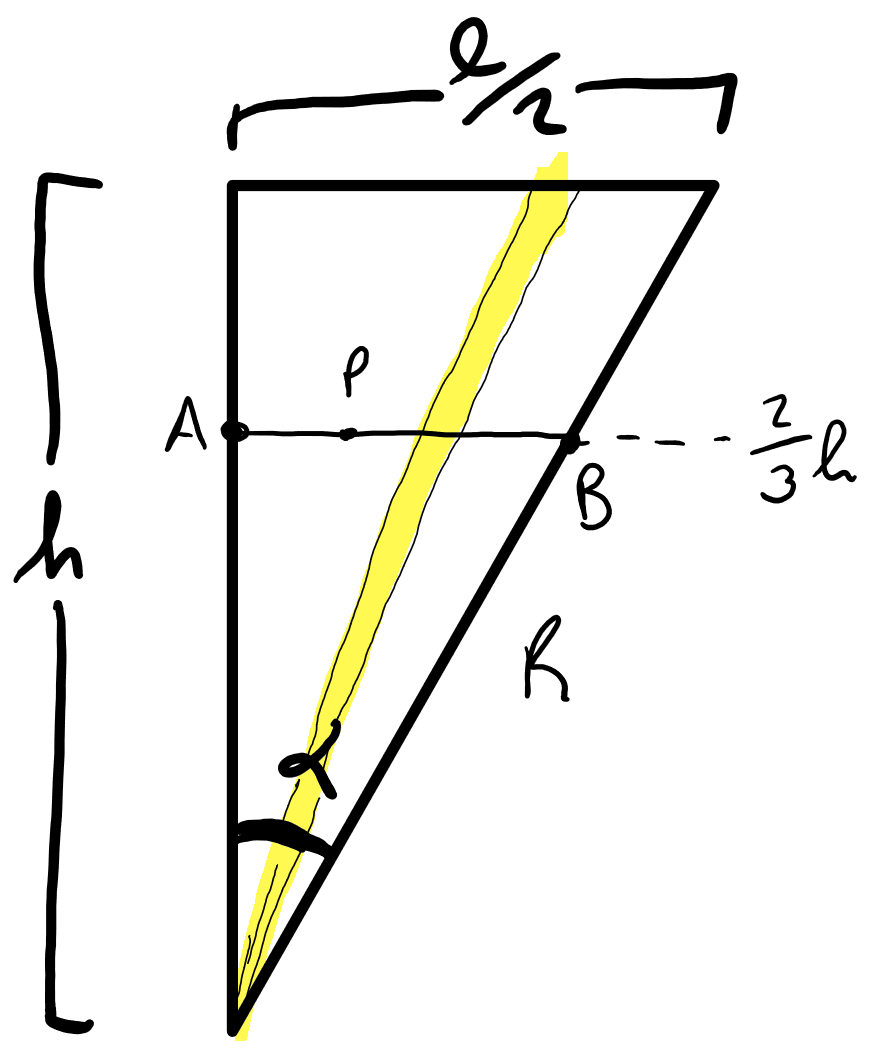
\includegraphics[width=0.25\textwidth]{meandist.png}
    \caption{(left) ; (center) ; (right) .}
    \label{fig:polygon}
\end{figure}

Given a regular polygon with $n$ sides (fig.~\ref{fig:polygon} left) the relationship between its area and the radius of the circumcircle can be determined from the following identities:
%
\begin{align*}
A &= \frac{\ell \cdot r}{2} \cdot n &
r &= R \cos \alpha &
\ell &= 2 \cdot R \sin \alpha &
\alpha &= \frac{2 \cdot \pi}{ 2 \cdot n} = \frac{\pi}{n}
\end{align*}
%
\begin{align}
A_n &= \frac{2 \cdot R \sin \alpha \cdot R \cos \alpha}{2} \cdot n = %\frac{R^2 \sin (2 \alpha)}{2} n \\
\frac{n}{2} \sin \left( \frac{2 \pi}{n} \right) R^2 \label{eq:area} \\
R_n &= \sqrt{ \frac{2 A}{n \sin \left( \frac{2 \pi}{n} \right)} } \label{eq:radius} 
\end{align}
%
The larger the number of edges the higher is the coverage of the reference circumscribed circle.
%
\begin{align*}
&A_3 = %\frac{3}{2} \sin \left( \frac{2 \pi}{3} \right) R^2 = \frac{3}{2} \cdot \frac{\sqrt{3}}{2} R^2
\frac{3 \sqrt{3}}{4} R^2 &\approx 1.299 \, R^2 \qquad\qquad &R_3 = \sqrt{ \frac{4 A}{3 \sqrt{3}}} &\approx 0.877 \, \sqrt{A} \\
&A_4 = %\frac{4}{2} \sin \left( \frac{2 \pi}{4} \right) R^2 = \frac{4}{2} R^2 =
2 R^2 &= 2.000 \, R^2 \qquad\qquad &R_4 = \sqrt{ \frac{A}{2}} &\approx 0.707 \, \sqrt{A} \\
&A_6 = %\frac{6}{2} \sin \left( \frac{2 \pi}{6} \right) R^2 = \frac{6}{2} \cdot \frac{\sqrt{3}}{2} R^2 =
\frac{3 \sqrt{3}}{2} R^2 &\approx 2.598 \, R^2 \qquad\qquad &R_6 = \sqrt{ \frac{2 A}{3 \sqrt{3}}} &\approx 0.620 \, \sqrt{A} \\
&A_\infty = \pi R^2 &\approx 3.142 \, R^2 \qquad\qquad &R_\infty = \sqrt{ \frac{A}{\pi}} &\approx 0.564 \, \sqrt{A}
\end{align*}


\subsection{Mean distance from center}

Possibly counter-intuitively, increasing the number of edges increases the covered area, but also the expected mean distance from the centre. For a certain bit budget, we can now compute maximum and expected error for a given tesselation.

\begin{align*}
A &= \frac{2}{3} \left( 0, h \right) &
B &= \frac{2}{3} \left( \frac{\ell}{2}, h \right) &
\frac{\ell}{2} &= R \sin \alpha &
h &= R \cos \alpha
\end{align*}

A more compact shape reduces the maximum absolute error, but makes the average mean distance from the centre.

\begin{align*}
P(t) &= (1-t) \cdot A + t \cdot B = \frac{2}{3} \left( t \cdot \frac{\ell}{2}, h \right) = \frac{2}{3} R \left( t \cdot \sin \alpha, \cos \alpha \right) \\
D(t) &= \frac{2}{3} R \sqrt{ t^2 \sin^2 \alpha + \cos^2 \alpha } \\
\overline{D} &= \int_{0}^{1} D(t) \, dt = \frac{2}{3} R \int_{0}^{1} \sqrt{ t^2 \sin^2 \alpha + \cos^2 \alpha } \, dt \\
&= \frac{1}{3} (R + R \cos \alpha \cot \alpha  \log (\tan \alpha + \sec \alpha ))
\end{align*}
%
This happens because more mass/area is distributed towards the perifery of the circumcircle (for details on the derivation see \cite{meandistance}).
\\

\begin{tabular}{lcccc}
\textbf{Reference shape}            & Triangle & Square & Hexagon & Circle \\
\textbf{Half-angle} $\mathbf{\alpha}$ (degrees)       & $60^\circ$ & $45^\circ$ & $30^\circ$ & $0^\circ$ \\
\textbf{Mean distance, unit radius} & 0.46 & 0.54 & 0.61 & $0.\overline{6}$
\end{tabular}


\subsection{Bit-budget vs. quality of approximation}

\begin{tabular}{lcccccccc}
\textbf{Base mesh} & T & O & C & T & O & C & T & O \\
\textbf{Subdivisions} & 20 & 20 & 20 & 21 & 21 & 21 & 22 & 22 \\
\textbf{Bit budget} & 41 & 42 & 42.6 & 43 & 44 & 44.6 & 45 & 46 \\
\textbf{Worst case approx.} & 9.45 & 6.68 & 6.22 & 4.72 & 3.34 & 3.11 & 2.36 & 1.67 \\
\textbf{Mean approximation} & 5.76 & 4.08 & 3.36 & 2.88 & 2.04 & 1.68 & 1.44 & 1.02
\end{tabular}


\begin{thebibliography}{1}

\bibitem{oblate} \href{https://en.wikipedia.org/wiki/Spheroid}{Spheroid (Wikipedia)}. \\ Retrieved on Jan 18th, 2016.

\bibitem{badastronomy} \href{http://blogs.discovermagazine.com/badastronomy/2008/09/08/ten-things-you-dont-know-about-the-earth}{Ten things you don't know about the Earth (BadAstronomy)}. \\ Retrieved on Jan 18th, 2016.

\bibitem{meandistance}
\href{http://www.mathpages.com/home/kmath283/kmath283.htm}{Mean Distance from Vertex to Interior of Plane Figures}. \\ Retrieved on Jan 18th, 2016.

\bibitem{lenofspherespiral} \href{https://www.intmath.com/blog/mathematics/how-to-find-the-length-of-a-spherical-spiral-10254}{How to find the length of a spherical spiral}. \\ Retrieved on Aug 24th, 2018.

\bibitem{spherespiralmodel} \href{https://mathematica.stackexchange.com/questions/136308/need-help-on-making-spiral-sphere-and-cone-helix}{Making a spiral sphere (MathExchange)}. \\ Retrieved on Aug 24th, 2018.

\bibitem{pointsonsphere} \href{http://blog.marmakoide.org/?p=1}{Spreading points on a disc and on a sphere}. \\ Retrieved on Aug 24th, 2018.

\bibitem{effdice} \href{https://www.eff.org/deeplinks/2016/07/new-wordlists-random-passphrases}{Deep Dive: EFF's New Wordlists for Random Passphrases}. \\ Retrieved on Aug 24th, 2018.

\bibitem{diceware} \href{http://world.std.com/~reinhold/diceware.html}{The Diceware Passphrase Home Page}. \\ Retrieved on Aug 24th, 2018.

\bibitem{PGPwordlist} \href{https://en.wikipedia.org/wiki/PGP_word_list}{PGP word list (Wikipedia)}. \\ Retrieved on Aug 24th, 2018.

\bibitem{plucodes} \href{https://plus.codes/developers}{Plus codes for developers}. \\ Retrieved on Aug 24th, 2018.

\bibitem{evaluation} \href{https://github.com/google/open-location-code/wiki/Evaluation-of-Location-Encoding-Systems}{Evaluation of Location Encoding Systems}. \\ Retrieved on Aug 24th, 2018.

\bibitem{opencodes} \href{https://github.com/google/open-location-code}{Open location codes (Github)}. \\ Retrieved on Aug 24th, 2018.

\end{thebibliography}

\end{document}
